% Created 2021-02-13 Sat 12:18
% Intended LaTeX compiler: pdflatex
\documentclass[11pt]{article}
\usepackage[utf8]{inputenc}
\usepackage[T1]{fontenc}
\usepackage{graphicx}
\usepackage{grffile}
\usepackage{longtable}
\usepackage{wrapfig}
\usepackage{rotating}
\usepackage[normalem]{ulem}
\usepackage{amsmath}
\usepackage{textcomp}
\usepackage{amssymb}
\usepackage{capt-of}
\usepackage{hyperref}
\author{Sam Barrett}
\date{\today}
\title{Log Week 2}
\hypersetup{
 pdfauthor={Sam Barrett},
 pdftitle={Log Week 2},
 pdfkeywords={},
 pdfsubject={},
 pdfcreator={Emacs 27.1 (Org mode 9.5)}, 
 pdflang={English}}
\begin{document}

\maketitle
This week I have:

\begin{itemize}
\item Re-read some papers, appreciating their approaches more now having attempted my own. Via different methods I have come to the same conclusions as a few of them.
\item Made my cooperative planning wrapper multi-threaded, increasing performance by \textasciitilde{}16x, it now pins all 16 cores to 100\% usage for the majority of the runtime. Scenarios which previously took upwards of 10minutes now take less than 1. This is useful from a research-viability standpoint but also allows me to run many more tests in the same space of time, increasing my productivity.
\item Tuned various parameters surrounding intersection and collision detection, reducing complexity whilst preserving effectiveness. More tuning is still required
\end{itemize}

Next week I intend to:

\begin{itemize}
\item Implement other genetic operators, specifically focusing on mutation to allow better exploration of challenging search spaces such as the one seen below, where an agent starting behind the vertical obstacle must explore far beyond the \emph{straight line optimal route} to find a route that does not pass through infeasible space.
\item Work on writing up my approach so far into my report.
\end{itemize}



\begin{center}
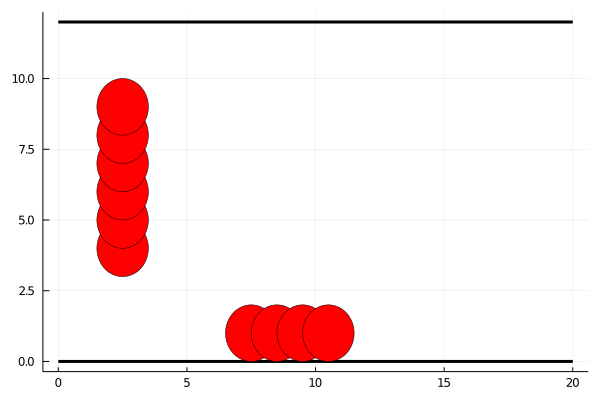
\includegraphics[width=.9\linewidth]{./road_graph.png}
\end{center}
\end{document}
